% Chapter 2
\chapter{Network on Chip (NoC)}
\label{chapter2}
%--------------------------------------------------------------------------
\section {Overview}
\hspace{5mm}Network on Chip (NoC) technology leverages the computer networking fundamentals for intra-chip and/or inter-chip communication between node/processing elements (PEs) and presents tremendous improvements over conventional bus and crossbar interconnections. Apart from these improvements, NoC implementation improves the scalability and repeatability of ASIC/SoC designs.\\


Many-core chip / multi-processors systems are increasingly being seen as the viable technique for high performance computing. Next generation of multi-core processors may contain hundreds of processors on a single chip. As the number of cores keeps rising, the on-chip communication infrastructure needs to be upgraded from the traditional bus architecture, which is the major performance bottleneck. NoC fundamentals are increasingly being seen as a possible alternative as it achieves the necessary trade-off between the cost-efficient but performance-limited bus architectures and performance efficient but cost/area inefficient point-to-point architectures. It can achieve a high degree of parallelism; however, since its design space is large, the designer is required to make intelligent design decisions to meet the quality of service (QoS) requirements.\\

At a high level, an NoC design methodology consists of a number of computational resources communicating with each other over a network infrastructure. The computational resources may include general purpose processing cores, DSP cores, specialized H/W modules, memory units such as RAMs, or even a heterogeneous combination of the above. The communication infrastructure consists of a set of interconnected routers (sometimes also referred to as ``switches") which relay the messages from the sending computational element (also referred to as processing element (PE)), in the form of smaller ``packets" and ``flits", to the destination computational element. In the NoC nomenclature, a ``packet" is the smallest unit used for routing and sequencing and may be composed of one or more ``flits". A flit (flow control digit) is the unit of bandwidth and storage, and is often also the smallest unit that can be transferred over a channel from one router to the other in a single cycle. It must be noted that a flit may be required to traverse over a number of network routers (which are also responsible for the routing decisions) before reaching the final destination. In effect, the routing of messages, in the form of smaller packets and flits, takes place on a network infrastructure, consisting of routers and interconnects between them, while the computational elements (connected to the network infrastructure through their associated routers) are only responsible for performing the required computations based on these messages. \\

Figure \ref{meshRouting} shows an example of a set of 16 routers connected in a Mesh topology, in which a flit sent by router 0 traverses through three other routers (1, 5 and 9) before reaching its final destination, namely router 10, in 3 clock cycles. In general number of clock cycles needed for a flit sent from one router to another is equal to the number or hops the flit goes before reaching the destination as each flit takes 1 cycles between two consecutive routers.

\begin{figure}[H]
	\centering
	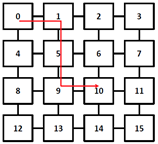
\includegraphics[scale=1]{./figs/meshRouting}
	\caption{Example of routing on NoC}
	\label{meshRouting}
\end{figure}

\section {NoC Design methodology }
\hspace{5mm}The NoC methodology is largely inspired by the established ``layered" approach in computer networks and effectively involves separation of application development from the communication infrastructure, thereby improving the design productivity and design time. The pioneering paper \cite{twelve} originally proposed the use of an on-chip network instead of global wiring for achieving communication between modules. In \cite{935594} further dwells on this idea and identifies the four layers in the NoC design methodology:

\begin{enumerate} 
	\item{\textbf{The Quasi-SERDES layer:} This layer specifies the width of the router buffers and channels. It also determines the flit-width. This layer is technology-dependent.}
	\item{\textbf{The data link layer:} This layer determines the protocol (for example single cycle or pipelined data transfer) between two interconnected routers. This is again technology-dependent. This layer may also incorporate error-checking. Any partitioning of NoC has to be done in this layer discussed later in the coming chapters.}
	\item{\textbf{The network layer:} This layer specifies the routing and forwarding mechanism of packets from the sender to receiver node. The processing nodes are indexed by the address bits (encoded within packets). This is again technology-dependent.}
	\item{\textbf{The transport layer:} This layer is responsible for bundling of messages into smaller ``packets" and ``flits" and also the appropriate addressing of source and destination nodes. This is often handled by the interfacing modules\cite{6498567}.}
\end{enumerate}

\hspace{5mm}As we enter the billion-gate era, the NoC design methodology significantly helps to improve the productivity, design cost and time-to-market in the following ways:
\begin{enumerate} 
	\item{The dissociation of communication and application layers and restricting the communication to standard interface enforces modularity in design, which also aids reuse of modules. It enables communication between heterogeneous modules and also imposes information hiding, since details of one module need not be known to the other for communicating messages. This has been explained in \cite{4550897}.}
	\item{The isolation of the network interface further reduces the test and verification costs.}
	\item{The NoC can be easily customized for a particular application to meet the timing and performance requirements.}
	\item{This is a scalable approach and can be easily extended to hundreds of communicating processing elements.}
\end{enumerate}

\hspace{5mm}In addition to the above, NoCs also find applications in cache coherency \cite{five}, Globally asynchronous locally synchronous (GALS) architectures \cite{fourteen}. We shall now discuss the four major considerations governing the design of a Network-on-Chip, as identified in \cite{4209016}, namely the NoC topology, routing, flow control and router micro-architecture:
\begin{enumerate} 
	\item{\textbf{Topology:} The topology of a network describes how the routers and the processing elements are connected in the network infrastructure \cite{6893205}. Most commonly explored NoC topologies in the literature include Ring, Mesh, Torus, Tree and butterfly. Topology can have a significant impact on the overall performance, as topology, together with routing strategy, determines the number of hops for message transmission. A topology often determines the cost of the NoC as it decides the number of PEs used and layout complexities involved. It may also have a significant bearing on the NoC power consumption, which is increasingly becoming a serious concern.}
	\item{\textbf{Routing:} The routing strategy determines how the packet is routed from its source to the final destination. The routing algorithm maybe}
	\begin{enumerate} 
		\item{\textbf{Deterministic,} in which the path from source to destination is always fixed (e.g. X-Y routing in Mesh),}
		\item{\textbf{Oblivious,} in which routing decisions maybe different for the same source and destination, however, the routing decision does not consider the state of the network (e.g minimal oblivious routing) or }
		\item{\textbf{Adaptive,} which uses local or global information about the network state to make decisions (e.g. PQ-routing, negative first routing).}
	\end{enumerate}
	
\hspace{5mm}The goal of the routing strategy is often to balance the load in a network, however, several routing strategies suffer from deadlock and the designer needs to be careful in choosing the right routing strategy.

	\item{\textbf{Flow Control:} The role of flow control is to regulate and manage the shared resources, such as buffer space, in the network. Since, unlike computer networks, the NoC is required to be lossless, the flow control protocol must also ensure that packets are not dropped and reliably delivered. Based on the granularity of resource allocation and bandwidth utilization, the flow control mechanisms are broadly classified as store-and forward, virtual-cut through, wormhole and virtual channel flow control. Flow control mechanism has a direct impact on the packet latency (and therefore Quality-of-Service or QoS), link utilization and complexity of router micro-architecture. The most commonly used flow control mechanisms for guaranteeing lossless behaviour of network are}
	\begin{enumerate} 
		\item{Credit-based flow control and}
		\item{Peek flow control (also referred to as on/off signalling)}
	\end{enumerate}
\hspace{5mm}In credit-based flow control, the sending routers maintain a credit count for each downstream router, which indicates the amount of available buffer space in the downstream routers. 
\hspace{5mm}In peek flow control, the downstream routers directly signal the buffer availability and the upstream routers are required to check this signal before forwarding flits. Peek flow control obviates the need for maintaining credit counters for available buffer space and also reduces the number of flow control signals \cite{connect_NoC}.
	\item{\textbf{Router micro-architecture:} The router micro-architecture deals with the actual circuit implementation of the router that helps in realizing the routing and flow control strategies. A typical router consists of a set of input ports connected to a routing logic, which determines the output port along which the flit/packet has to be forwarded. The flits are stored in buffers before being scheduled by the arbitration logic to the switching network, after considering the buffer space availability in the downstream buffers. The switch finally helps the packet depart the router through the selected output port. Additionally, each port (input and output) has flow control signals associated to it. Figure \ref{routerMicroArchitecture} show a typical router micro-architecture. Sometimes, the router data path is pipelined to improve the clock speed. Router complexity is influenced by the number of incoming/outgoing ports and the flow control and routing logic.}
	\begin{figure}[H]
		\centering
		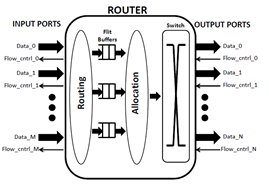
\includegraphics[scale=1]{./figs/routerMicroArchitecture}
		\caption{\textbf{A typical router micro-architecture \cite{yatish_ddp}}}
		\label{routerMicroArchitecture}
	\end{figure}
	
	\item{\textbf{Buffering:} Buffering is the strategy used to store information and ensure that no data is lost in the transiting flits between routers when router is busy and not ready to accept data in a situation when there is congestion in the network, and the packet cannot be forwarded immediately to the correct port. Buffer can be single buffer per router shared by all input ports or it can be single buffer per port, it's most common implementation is in the form of FIFO. In this system, NoC uses XY routing, which is deterministic and static routing, Round Robin arbitration, which is distributed and dynamic arbitration approach, and multiple buffers (typically 8) at each input port of the router using FIFO.}
\end{enumerate}

\hspace{5mm}The routers at each level share a similar functionality i.e. routing and handling packets protocol. The port indicates a direction to/from the group, the cluster or the system root. This port can be connected only to the router of the same level or the gateway to the higher level of the hierarchy. If this port is not connected, the router acts as a system root and discards packets of unknown destination. That means that the input port can be connected to the output port of another router at the same level or to the group gateway. Additionally, in case of a local network, the input port may be connected to the application end point.

\section{CONNECT for network generation}
\hspace{5mm}CONfigurable Network Creation Tool \cite{connect_NoC_tool} created by Michael Papamichael of Computer Science Department, Carnegie Mellon University, provides an FPGA friendly fully synthesizable NoC. This RTL design of a NoC can be automatically generated using the web based interface for any desired topology and node count. CONNECT supports a variety of common network topologies, as well as custom user configured networks, that can be either specified through special configuration files or created through the CONNECT Network Editor. A variety of network and router parameters, such as the router type, pipe-lining options, the number of virtual channels or allocator type, allow the user to further customize the network and trade-off between resource usage and performance to satisfy application-specific requirements. Refer to README document in CONNECT generated NoC directory for details. Figure \ref{connectMeshFig} is a network generated using CONNECT network generation tool.
\begin{figure}[H]
	\centering
	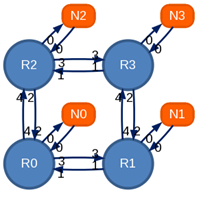
\includegraphics[scale=1]{./figs/connectMeshFig}
	\caption{\textbf{2 $\times$ 2 Mesh topology NoC generated using CONNECT}}
	\label{connectMeshFig}
\end{figure}

\hspace{5mm}Each of these nodes is associated with a routing table which directs the incoming data know as a flit to a particular output port based on the input address flagged in the flit packet. The flit format is as shown in figure \ref{flit_structure}below

\begin{figure}[H]
\centering
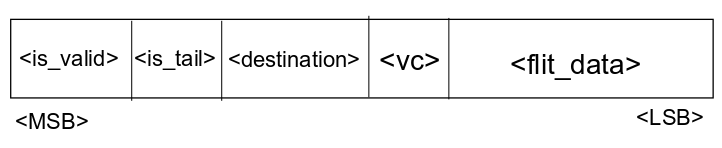
\includegraphics[scale=0.5]{./figs/flit_structure}
\caption{CONNECT NoC Flit structure}
\label{flit_structure}
\end{figure}

\textbf{$<$valid bit$>$:} Indicates a valid flit. Set to 1 when sending a flit. \newline

\textbf{$<$tail bit$>$:} Indicates this is a tail flit, i.e. the last flit of a packet. Set high for single-flit packet as they are also tail flits. \newline

\textbf{$<$destination$>$:} Specifies the destination of the current flit. Populate with a valid binary encoded router ID that corresponds to one of the routers in the network. \newline

\textbf{$<$virtual channel$>$:} For Virtual channel based networks this field specifies the virtual channel to use and should be populated with a valid VC, depending on the number of available virtual channels. We use a non-VC based NoC in our project. Therefore, VC bit is set as ‘0’. \newline \

\textbf{$<$data$>$:} User data field. Populate with data to be transferred. \newline \newline
The Table \ref{NoC_parameters} display the parametric setting while using CONNECT. 

\begin{table} [H]
\caption{NoC Parameters}
\centering
\begin{tabular}{||c | c||} 
\hline
	Topology 		& Mesh 				   \\ 
	Routers per Row 	& 4 				   \\
	Routers per Column 	& 4				   \\
	Router Type 		& Virtual Channel (VC) 		   \\
	Number of VCs 		& 2 				   \\
	Flow Control Type 	& Credit-Based Flow Control 	   \\
	Flit Data Width 	& 64 				   \\
	Flit Buffer Depth 	& 8 				   \\
	Allocator 		& Separate-Input First Round-Robin \\
\hline
\end{tabular}
\label{NoC_parameters}
\end{table}

To understand the data transfer and working of generated NoC let us work out a simple example where a flit injected into node zero of Figure \ref{connectMeshFig} to destination node 4, here we just need to keep a note of the specified destination bit in the flit in the flit format. Router 0 looks up in the routing Table \ref{Router_Destinations} and puts the flit to the appropriate port, in this case port 4. Now the flit is received at the port 4 of router 2 which is again directed to port 3, which is received at port 3 of router 3. Finally looked up in the routing table and is presented in port 0 of router 3. The transfer of the flit from source to destination is now complete. The cost of the transfer in terms of number of clocks required is equal to the number of routers flit passes through to before it reaches the destination. In this case no. of clock cycles required by the flit from source to destination is 3 clock cycles.

\begin{table} [H]
\caption{Router Destinations}
\begin{center}
\begin{tabular}{||c | c | c | c | c||} 
\hline
	Destination &   Router 0 &   Router 1 &   Router 2 &   Router 3 \\ \hline
	    0 	    &   Port 0   &   Port 1   &   Port 2   &   Port 2   \\
	    1 	    &   Port 3   &   Port 0   &   Port 2   &   Port 2   \\
	    2 	    &   Port 4   &   Port 1   &   Port 0   &   Port 1   \\
	    3 	    &   Port 4 	 &   Port 4   &   Port 3   &   Port 0   \\ \hline
\end{tabular}
\end{center}
\label{Router_Destinations}
\end{table}

\section {NoC Performance Parameters}
The performance of any NoC can be evaluated by three parameters:
\begin{enumerate}
 \item \textbf{\textit{Latency:}} Latency is the time elapsed between  the beginning of transmission of message. Latency is the basis for comparison among different design choices. It can be expressed in terms of simulator clock cycles. The CONNECT \cite{connect_NoC} NoC (under no traffic condition) has the maximum latency of $2$ clock cycles between two adjacent routers and $n+2$ clock cycles, if there are $n$ numbers of routers in the path or XY routing.
 \item \textbf{\textit{Throughput:}} Throughput is defined as the maximum amount of information delivered per unit time. The unit of measure is messages per second or messages per clock cycles or bits per clock cycle. The CONNECT \cite{connect_NoC} NoC has the latency term given by $n+2$, in which $n$ has co-efficient = $1$, Hence, at any router maximum throughput is $1\ flit/cycle$ 
 \item \textbf{\textit{Bandwidth:}} The maximum rate of data propagation once the data is in the network. The unit of measure is bits per second (bps). Bandwidth (in bps) depends on the maximum operating frequency of NoC, and hence on the platform on which it is implemented (i.e. FPGA or ASIC) 
\end{enumerate}
\newpage
\section{Test Cases}
\begin{enumerate}
\item{\textbf{Best Case:} Each node sends a flit at each clock edges to every other node. 
The test bench fragment below send a single flit to a 4 $\times$ 4 mesh type NoC node at different clock cycles to every other node in the NoC one by one.}
\begin{lstlisting}
	for(x = 15; x >= 0; x = x - 1)
	begin
		for(y = 15; y >= 0; y = y - 1 )
		begin
			#(ClkPeriod);
			start = 1'b1;
			send_flit[x] = 1'b1;
			vc = 0;
			data = data + 1;
			flit_in[x] = {1'b1 /*valid*/, 1'b0 /*tail*/, y[3:0], vc, data};
			$display("Injecting flit %x into send port %0d of router %0d to router %0d", flit_in[x], x, x, y);
			#(ClkPeriod);
			send_flit[x] = 1'b0;
			flit_in[x] = {1'b0 /*valid*/, 1'b0 /*tail*/, y[3:0], vc, data};
			wait (flit_out[y] == {1'b1,flit_in[x][16:0]});
			start = 1'b0;
			$display("Receiving flit %x at receive port of router = %0d in %0d us", flit_out[y], y, z*10);
			#(HalfClkPeriod);
		end
	end
\end{lstlisting}
\item{\textbf{Average Case:} Any one node sends a flit at each clock edges to another node \\
The average case is when there is not more than one flit received by any node in in the NoC. This case is easily verifiable by slight modification of above code fragment.}
\item{\textbf{Worst Case:} Multiple nodes send a flit to a single router at the same clock cycle\\
The test bench fragment below send a data flit from node 1 and node 4 to node 0 every clock cycles. This makes the internal out port buffer of node 0 to overflow and hence flit are lost. To prevent this we have to stop sending data when buffer is not ready to accept data which is indicated by \textbf{send\_ports\_0\_getNonFullVCs} of the sending node. }
\begin{lstlisting}
	for(x = 0; x <= 50; x = x + 1)
	begin
		//#(HalfCLKPeriod);
		start = 1'b1;
		send_flit[1] = 1'b1;
		vc = 0;
		flit_in[1] = {1'b1 /*valid*/, 1'b0 /*tail*/, 4'b0, vc, data1};
		send_flit[4] = 1'b1;
		vc = 0;
		data1 = data1 - 1;
		data2 = data2 + 1;
		flit_in[4] = {1'b1 /*valid*/, 1'b0 /*tail*/, 4'b0, vc, data2};
		$display("Injecting flit %x into send port %0d of router %0d to router %0d\nAnd\nInjecting flit %x into send port %0d of router %0d to router %0d ", flit_in[1], 1, 1, 0, flit_in[4], 4, 4, 0);
		#(CLKPeriod);
		send_flit[1] = 1'b0;
		send_flit[4] = 1'b0;
		flit_in[1] = {1'b0 /*valid*/, 1'b0 /*tail*/, 4'b0, vc, data1};
		flit_in[4] = {1'b0 /*valid*/, 1'b0 /*tail*/, 4'b0, vc, data2};
	 end
\end{lstlisting}
\end{enumerate}

In the next chapter we shall discuss the methods of NoC partitioning and the ways to automate the process. The chapter will also discuss a few test cases showing the comparison between an un-partitioned and a partitioned NoC. 